\subsection{序关系与基数上的运算}

命题13. 设 \(\mathfrak{a}\) 与 \(\mathfrak{b}\) 是基数。则 \(\mathfrak{a} \geqslant \mathfrak{b}\) 当且仅当存在一个基数 \(\mathfrak{c}\) 使得 \(\mathfrak{a} = \mathfrak{b} + \mathfrak{c}\) .

因为关系 \(a \geqslant b\) 意味着存在a的一个与b等势的子集B（第2号），即a与b和某个集合c所成的和集等势。

\pandocbounded{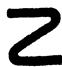
\includegraphics[keepaspectratio]{images/part002_f1d2aad8dae595af04a38c0526d2ebc1f30c28017ae785c1fe861e266dceeae2.jpg}}

如果 \(a \geqslant b\) ，通常存在许多基数 \(c\) 使得 \(a = b + c\) （参见§6）；因此，一般来说，不可能定义两个这样的基数的“差” \(a - b\) （参见§5，第2号）。

命题14。设 \((\mathfrak{a}_i)_{i\in I}\) 与 \((\mathfrak{b}_i)_{i\in I}\) 是两族基数，它们都由同一个集合 \(I\) 索引，并且使得 \(\mathfrak{a}_i\geqslant \mathfrak{b}_i\) （对于所有 \(i\in I\) ）。则

\[
\sum_ {i \in I} a _ {i} \geqslant \sum_ {i \in I} b _ {i}, \quad \mathbf {P} _ {i \in I} a _ {i} \geqslant \mathbf {P} _ {i \in I} b _ {i}.
\]

第二个不等式由集合乘积之间的包含关系得出（第二章，§5，第4号，命题6，推论3）。至于第一个不等式，如果集合E是某个族 \((\mathbf{A}_{t})_{t\in\mathbf{I}}\) 的互不相交子集的并集，且如果 \(B_{t}\subset A_{t}\) 对于所有 \(t\in I\) ，则 \(B_{t}\) 也是两两不相交的，并且 \(\bigcup_{i}B_{i}\subset\bigcup_{i}A_{i}\) （第二章，§4，第2号）。

推论1. 设 \((\mathfrak{a}_i)_{t \in I}\) 为一族基数。对于每个子集 \(J\) （ \(I\) 的子集），我们有 \(\sum_{i \in J} \mathfrak{a}_i \leqslant \sum_{i \in I} \mathfrak{a}_i\) 。如果还有 \(\mathfrak{a}_i \neq 0\) （对于所有 \(i \in I - J\) ），那么 \(\mathsf{P}_{i \in J} \mathfrak{a}_i \leqslant \mathsf{P}_{i \in I} \mathfrak{a}_i\) 。置 \(\mathfrak{b}_i = \mathfrak{a}_i\) （若 \(i \in J\) ），以及 \(\mathfrak{b}_i = 0\) （相应地， \(\mathfrak{b}_i = 1\) ）（若 \(i \in I - J\) ）。然后应用命题14，并注意到关系 \(\mathfrak{a} \neq 0\) 蕴含 \(\mathfrak{a} \geqslant 1\) .

推论2。如果 \(\mathfrak{a}\) , \(\mathfrak{a}'\) , \(\mathfrak{b}\) , \(\mathfrak{b}'\) 是基数，使得 \(\mathfrak{a} \leqslant \mathfrak{a}'\) , \(\mathfrak{b} \leqslant \mathfrak{b}'\) ，以及 \(\mathfrak{a}' > 0\) ，那么 \(\mathfrak{a}^{\mathfrak{b}} \leqslant {\mathfrak{a}'}^{\mathfrak{b}'}\) .

由命题10和命题14可得 \(a^b \leqslant a'^b\) ，由命题10和命题14的推论1可得 \(a'^b \leqslant a'^{b'}\) 。

定理2（康托尔）。对于每个基数a，我们有 \(2^{\mathfrak{a}} > \mathfrak{a}\) .

我们有 \(\operatorname{Card}(\mathfrak{P}(\mathfrak{a})) = 2^{\mathfrak{a}}\) （第5号，命题12）。映射 \(x \to \{x\} (x \in \mathfrak{a})\) 是 \(\mathfrak{a}\) 到 \(\mathfrak{P}(\mathfrak{a})\) 中的一个单射，由此 \(\mathfrak{a} \leqslant 2^{\mathfrak{a}}\) 。因此只需证明 \(\mathfrak{a} \neq 2^{\mathfrak{a}}\) ，即对于每一个映射 \(f\) （从 \(\mathfrak{a}\) 到 \(\mathfrak{P}(\mathfrak{a})\) 中的映射），图像 \(f(\mathfrak{a})\) 都不同于 \(\mathfrak{P}(\mathfrak{a})\) . 设 \(\mathbf{X}\) 是所有 \(x \in \mathfrak{a}\) （满足 \(x \notin f(x)\) ）所成的集合。如果 \(x \in \mathbf{X}\) ，我们有 \(x \notin f(x)\) ，由此 \(f(x) \neq \mathbf{X}\) ；若 \(x \in \mathfrak{a} - \mathbf{X}\) ，我们有 \(x \in f(x)\) 并且 \(x \notin \mathbf{X}\) ，由此 \(f(x) \neq \mathbf{X}\) 。这表明 \(\mathbf{X} \notin f(\mathfrak{a})\) 并证明了该定理。

推论。不存在一个集合，它以每个基数作为元素。

如果U是这样的集合，那么就会存在一个集合S，它是集合族 \((\mathbf{X})_{\mathbf{x}\in\mathbf{U}}\) 的和，使得每个基数都与S的某个子集等势。特别地，设 \(\mathfrak{S}=\operatorname{Card}(\mathbf{S})\) ；由于 \(2^{S}\) 是一个基数，我们就会有 \(2^{S}\leqslant S\) ，这与定理2矛盾。

